\chapter{Introduction }
\paragraph{}Over the past decade, benefiting from the rapid
development of wireless communication technology, sensing
technology and the improvement of big data analysis
capacity [1], the Internet of Things (IoT) is growing with
incredible speed in most areas, especially in healthcare [2],
smart city [3] and autonomous vehicles [4]. As the essential
elements of the IoT world, data collected from various
devices can be applied in a wide range of areas after being
analyzed and processed. Combining with advanced
technologies such as big data and artificial intelligence [5],
IoT service based on data not only reduces the cost of industry and agriculture and makes the devices around
people more intelligent, but also repeatedly optimizes the
IoT ecosystem (security, equipment management and the
standardization [6]) itself. However, due to the limited high
maintenance and management cost [7], restricted collecting
scope in privacy data, data exchange between individual and
organizations become irreversible trend when they realize
that connection is more important than possession [8].
Therefore, a lot of data exchange or sharing platform hava
emerged in the past years. Such as crawdad for archiving
wireless data [9], data science central provided industry’s
online resources for big data practitioners, data.gov as the
home of the US government’s open data platform, the
development of digital coast met the unique needs of the
coastal management community [10,11]. Most of them
concentrated on data of the same kind or a specific field and
led by government or the unions of large institutions.
However, the data sets on such centralized platform cannot
meet the public’s diversified demands, largely due to they
cannot provide enough trust to guarantee the transparency,
auditable, immutable in data exchange process.
\paragraph{}It has been watched by researchers for a long time, as the issue of trust kills the enthusiasm to share data actively and seriously hampers the development of the data industry [12]. Although current platforms integrate a lot of confidentiality mechanisms (access control, authorization privacy) and propose some trust model for data sharing in IoT, they are not break away from the third party [13].
\paragraph{}In order to guarantee IoT data exchange in a completely trusted, transparent environment, we propose a decentralized solution based-on blockchain. As the core technology inBitcoin, blockchain soon came to be widely attracted attention and application for its trust property[14].
\paragraph{}The core advantage of blockchain is decentralization. It consists of data encryption, timestamp, distributed consensus algorithm, economic incentive mechanism and other technology. It is applicable to the point-to-point transaction based on decentralized credit in distributed systems without mutual trust. Sequentially, this technology solves the prevailing high cost, low efficiency and uneasiness of data storage in current central institutions. This paper utilizes the feature of data is not tampered and completely transparent, combines with the time stamp and the transaction details in the process of storage and trading, so that it can be trusted by many parties. Its mixed encryption technology based on asymmetric encryption makes the user's privacy information secure with the public and private key as the only identifier of transaction subject. The second generation blockchain introduces intelligent contract, which makes the blockchain easier to use distributed application programming and speed up transaction speed. The Ethereum intelligent contract combined with capability-based access control method
makes the data provider can completely control their own
data sharing permissions quickly and efficiently and
completely solve the credible issues of original system in the
data.

\chapter{A Step to Blockchain}

\section{Blockchain data structure}

\subsection{Structure of a block}

\paragraph{}A blockchain, is a growing list of records, called blocks, which are linked using cryptography. Each block contains a cryptographic hash of the previous block, a timestamp, and transaction data (generally represented as a merkle tree root hash).
A block is a container data structure, which brings together transactions for inclusion in the public ledger, known as the blockchain. The block is made up of a header; containing metadata, followed by a long list of transactions. A block can be identified in two ways, either by referencing the block hash, or through referencing the block height. The block header consists of three sets of block metadata. Metadata is data that provides information about other data. Firstly, there is a reference to a previous block hash, which connects this block to the previous block, lying in the blockchain. The second set of metadata relates to the mining competition; namely the difficulty, timestamp and nonce. Lastly, the third piece of metadata is the Merkle Tree root; a data structure used to summarize all the transactions in the block in an efficient manner.
\paragraph{}Block headers can be regarded as an example of a dynamic membership multi-party signature (DMSS). A DMSS is a digital signature formed by a set of signers which has no fixed size (Back, Corallo, Dashjr, & Friedenbach, 2014).Bitcoin’s block headers are DMSS because their proof of work has the property that anyone can contribute without undergoing an enrolment process. Furthermore, contribution is weighted by proportional computational power rather than one threshold signature contribution per party (Back, Corallo, Dashjr, & Friedenbach, 2014). This allows anonymous membership without risk of a Sybil attack. A Sybil attack is when one party joins many times and has an uneven, disproportionate input into the signature. Since the blocks are chained together, Bitcoin’s DMSS is cumulative. A chain of block headers is also a DMSS on its first block, with computational strength equivalent to the sum of the computational strengths of the composing DMSS . Therefore, the key innovation in Blockchain is a signature of computational power, rather than the typical signature of knowledge.

\begin{figure}[H]
	\centering
	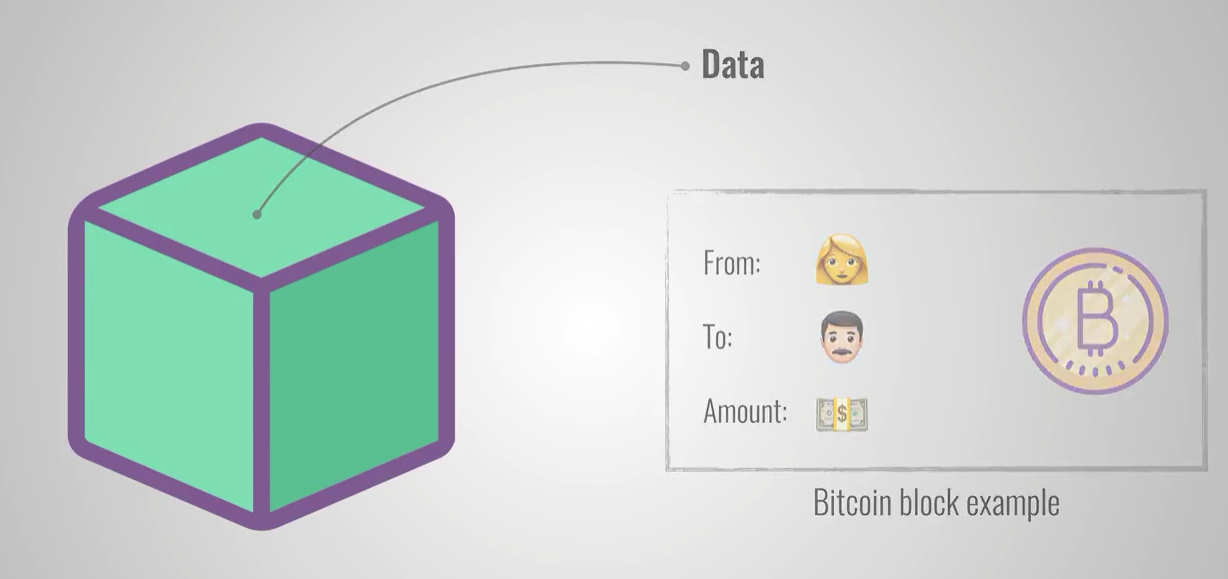
\includegraphics[scale=0.2]{data_block.png}
	\caption{Data in the Block}
\end{figure}

\begin{figure}[H]
	\centering
	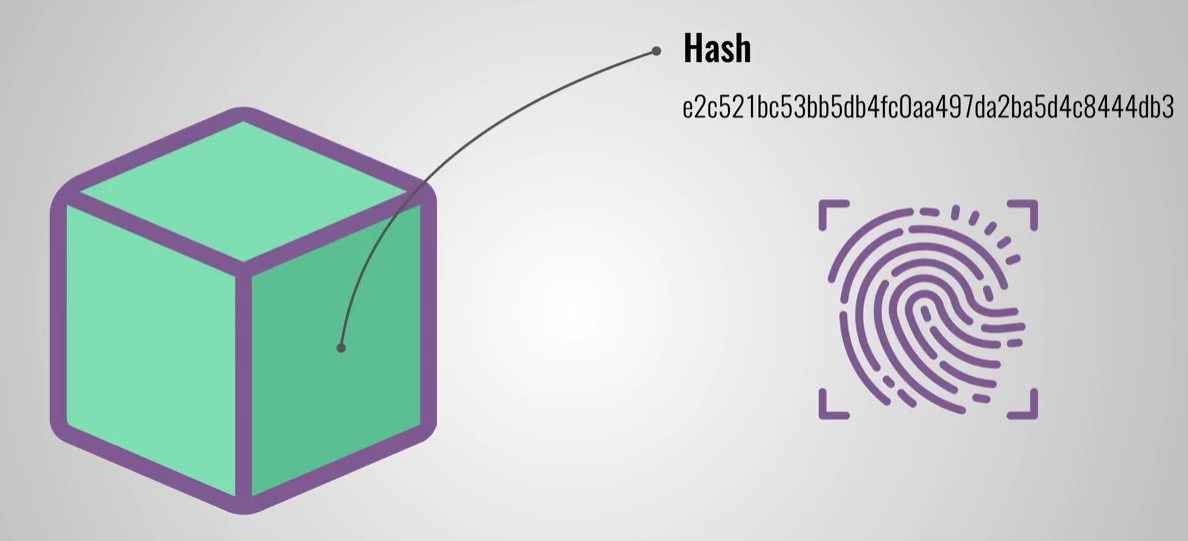
\includegraphics[scale=0.2]{hash_block.png}
	\caption{Hash in the Block}
\end{figure}

\begin{figure}[H]
	\centering
	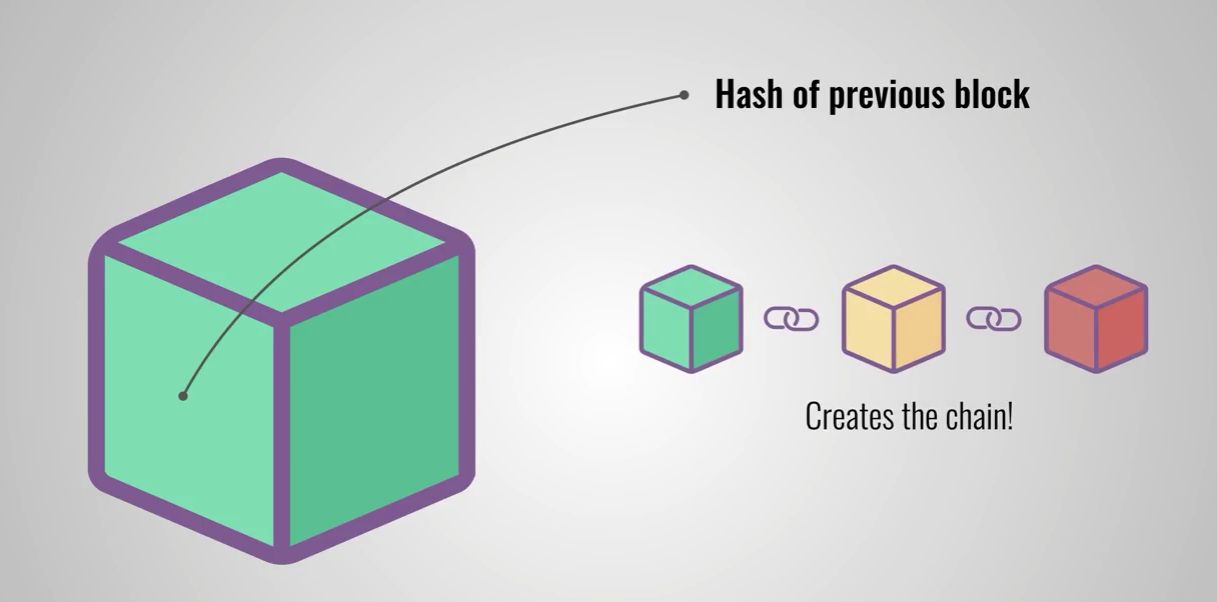
\includegraphics[scale=0.2]{previous_block.png}
	\caption{Hash of the Previous Block}
\end{figure}

\subsection{Block header hash and nodes}

\paragraph{}Here I have am providing an example, the block hash of the first Bitcoin block ever created will be like 000000000019d7789c085ae165831e934gf763ae46a4a6c172b3f1b60a8ce26f. The block hash identifies a block uniquely, and can be independently derived by any node simply by hashing the block header. A node is a full client. A full client is a client that owns the block chains and is sharing blocks and transactions across the blockchain network. A node is considered to be part of the blockchain infrastructure, and does not necessarily have to be a miner. Each node keeps a complete copy of a totally ordered sequence of events in the form of a blockchain . The block’s hash is computed by each node, as the block is received from the network. The block hash may be stored in a separate database table as part of the block’s metadata, to facilitate indexing and faster retrieval of blocks from disk.

\subsection{Block height}

\paragraph{}Block height is another method to identify a block, this time through its position in the blockchain. The first block ever created is at block height 0 (zero), and in the case of Bitcoin, is the same block that was referenced by the block hash of the above block which is 000000000019d7789c085ae165831e934gf763ae46a4a6c172b3f1b60a8ce26f .Each subsequent block added “on top” of that first block is one position “higher” in the blockchain, like boxes stacked one on top of the other.Block height does not always identify a particular singular block. It is possible for two or more blocks may have the same block height, both competing for the same position in the blockchain.

\subsection{Genesis Block}

\paragraph{}The first block in any blockchain is termed the genesis block. If you start at any block and follow the chain backwards chronologically, you will arrive at the genesis block. The genesis block is statically encoded within the client software, that it cannot be changed. Every node can identify the genesis block’s hash and structure, the fixed time of creation, and the single transactions within. Thus every node has a secure “root” from which is possible to build a trusted blockchain on.

\subsection{Proof of Work}

\paragraph{}In Proof of Work, in order for an actor to be elected as a leader and choose the next block to be added to the blockchain they have to find a solution to a particular mathematical problem.
Given that the hash function used is cryptographically secure, the only way to find a solution to that problem is by bruteforce (trying all possible combinations). In other words, probabilistically speaking, the actor who will solve the aforementioned problem first the majority of the time is the one who has access to the most computing power. These actors are also called miners.
\paragraph{}It has been widely successful primarily due to its following properties:

\begin{enumerate}
  \item It is hard to find a solution for that given problem
  \item When given a solution to that problem it is easy to verify that it is correct.
\end{enumerate}

\paragraph{} Whenever a new block is mined, that miner gets rewarded with some currency (block reward, transaction fees) and thus are incentivized to keep mining. In Proof of Work, other nodes verify the validity of the block by checking that the hash of the data of the block is less than a preset number.Due to the limited supply of computational power, miners are also incentivized not to cheat. Attacking the network would cost a lot because of the high cost of hardware, energy, and potential mining profits missed.

\subsection{Linking blocks in the blockchain}

\paragraph{}Nodes maintain a copy of the blockchain locally, starting from the genesis block. The local copy of the blockchain constantly updates as new blocks are discovered and subsequently built on the chain. As a node receives information of incoming blocks from the network, it will validate these blocks first, then link them to the existing blockchain.The process to establish a link is as follows; a node will examine the incoming block header and look for the “previous block hash”. Looking at this incoming block, the node finds the “previous block hash” field, which contains the hash of its parent block. This hash is known to the node previously. Therefore, the node reasons that this new block is a child of the last block on the chain, and is the legitimate extension of the chain. The node adds this new block to the end of the chain, making the blockchain longer with a new height of the incoming block, now validated.

\section{Cryptographic Hash Algorithm}

\paragraph{}The blockchain data structure is a back-linked list of blocks of transactions, which is ordered. It can be stored as a flat file or in a simple database. Each block is identifiable by a hash, generated using the SHA256 cryptographic hash algorithm on the header of the block. Each block references a previous block, also known as the parent block, in the “previous block hash” field, in the block header.A hash, also known in long form as cryptographic hash function, is a mathematical algorithm that maps data of arbitrary size to a bit string of a fixed size. In the case of SHA 256, the result is a string of 32 bytes. The resultant 32 bytes makes it effectively impossible to reverse the output, since the function was designed to be a one-way function .

\paragraph{}The idea behind a hash functions use is to facilitate a thorough means for searching for data in a dataset. The most basic form of hash function is any function that can be used to map data of arbitrary size to data of fixed size. This output is a bit-string known as the hash value, hash sum or hash code. The hash values can be stored in a tabular form known as a hash table and is an efficient indexing mechanism; especially useful in search performance. Hash functions are collision-free too. That means it’s impossible to find two messages that hash to the same hash value. Therefore, when given a compact hash, one can confirm that it matches a particular input datum. Blocks can be identified from their hash, serving two purposes; identification and integrity verification.
 
 \paragraph{}Bitcoin hashing function makes use of the SHA 256, applied twice. It generates an almost-unique, fixed size 256-bit (32-byte) hash security. Large classes of hash functions are based on a building block of a compression function .Each block contains the hash of its parent inside its own header. There lays a chain going all the way back to the first block created, also known as the genesis block, linked together by a sequence of hashes. The “previous block hash” field is inside the block header and thereby the current block hash is dependent on the parent block hash. The child’s own identity changes if the parent’s identity changes. When the parent is modified in any way, the parent’s hash changes. The parent’s changed hash necessitates an alteration in the “previous block hash” pointer of the child. This in turn causes the child’s hash to mutate, which requires a change in the pointer of the grandchild, which in turn alters the grandchild and so on.
 
\paragraph{}This cascading effect ensures that, once a block has many generations succeeding it, it cannot be changed without consequently forcing a recalculation of all the subsequent blocks. Because such a recalculation would require an enormous amount of computation, the existence of a long chain of blocks fortifies the Blockchain’s deep history to be immutable; a key feature of blockchain technology security.

\section{Modification of Data}
\paragraph{}By design, a blockchain is resistant to modification of the data. It is "an open, distributed ledger that can record transactions between two parties efficiently and in a verifiable and permanent way". For use as a distributed ledger, a blockchain is typically managed by a peer-to-peer network collectively adhering to a protocol for inter-node communication and validating new blocks. Once recorded, the data in any given block cannot be altered retroactively without alteration of all subsequent blocks, which requires consensus of the network majority. Although blockchain records are not unalterable, blockchains may be considered secure by design and exemplify a distributed computing system with high Byzantine fault tolerance. Decentralized consensus has therefore been claimed with a blockchain.

\paragraph{}Blockchains are incredibly popular nowadays.Here, I have a chain of three blocks. As you can see, each block has a hash and a hash of the previous block.So block 3 points to block 2 and block 2 points to the block 1. Now the block 1 is special. It is the Genesis block and it cannot point to any other block. Now if block 2 is tampered, it changes the hash of the block 2. Now the hash in the block 3 becomes invalid as it does not match with the hash in the previous block. Computers are very fast and they can calculate hash at a very high speed.

\begin{figure}[H]
	\centering
	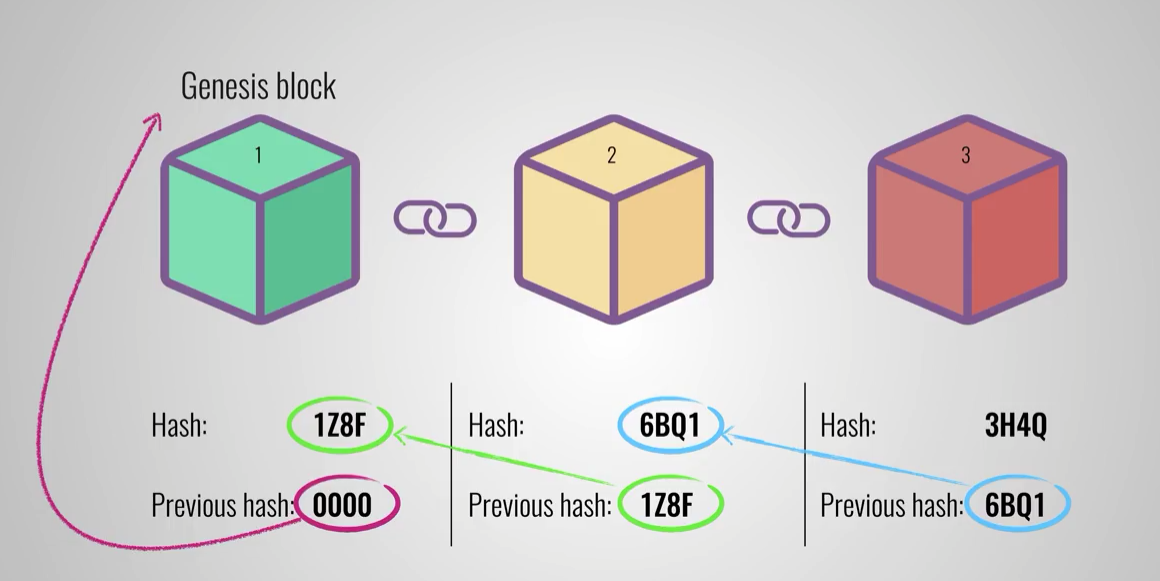
\includegraphics[scale=0.3]{total_block.png}
	\caption{Chaining the blockchain}
\end{figure}

\begin{figure}[H]
	\centering
	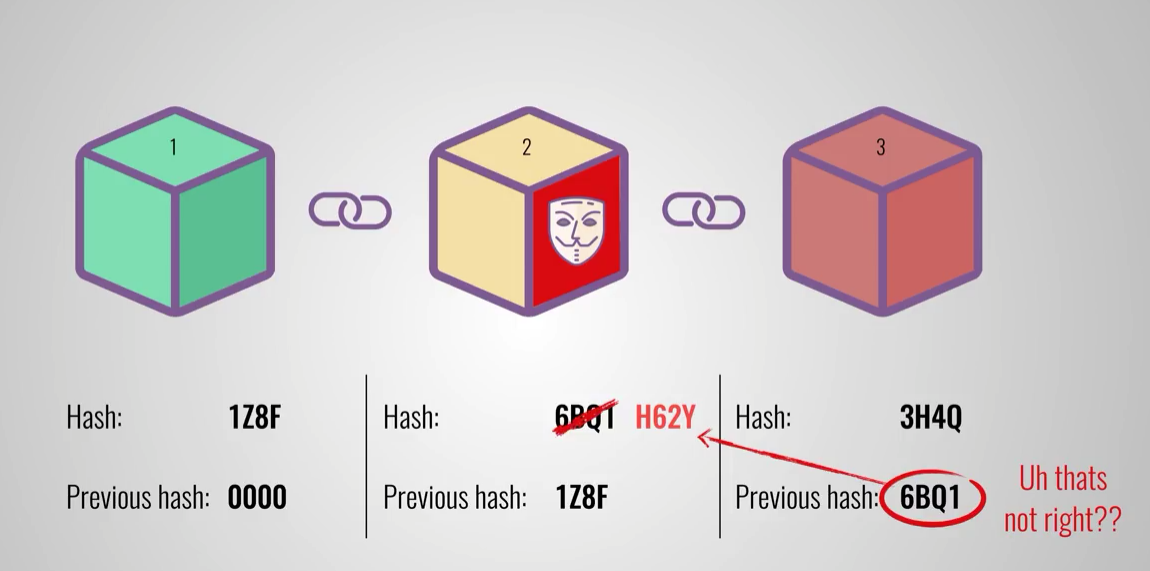
\includegraphics[scale=0.3]{tampering_block.png}
	\caption{Denial on Data Modification}
\end{figure}

\section{Types of blockchains}

\begin{itemize}
    \item {Public blockchains}\textbf{ : }A public blockchain has absolutely no access restrictions. Anyone with an internet connection can send transactions[disambiguation needed] to it as well as become a validator (i.e., participate in the execution of a consensus protocol). Usually, such networks offer economic incentives for those who secure them and utilize some type of a Proof of Stake or Proof of Work algorithm.Some of the largest, most known public blockchains are Bitcoin and Ethereum.
    
    \item {Private blockchains}\textbf{ : }A private blockchain is permissioned. One cannot join it unless invited by the network administrators. Participant and validator access is restricted.This type of blockchains can be considered a middle-ground for companies that are interested in the blockchain technology in general but are not comfortable with a level of control offered by public networks. Typically, they seek to incorporate blockchain into their accounting and record-keeping procedures without sacrificing autonomy and running the risk of exposing sensitive data to the public internet.
    
    \item {Consortium blockchains}\textbf{ : }A consortium blockchain is often said to be semi-decentralized. It, too, is permissioned but instead of a single organization controlling it, a number of companies might each operate a node on such a network. The administrators of a consortium chain restrict users’ reading rights as they see fit and only allow a limited set of trusted nodes to execute a consensus protocol.

\end{itemize}

\section{Applications}

\begin{itemize}
    \item The Food Industry
    \item Cyber Security
    \item Voting
    \item Land Registry
    \item Smart Contracts
    \item Banks
    \item Insurance
    \item Internet-of-Things (IoT)
    \item Smart Appliances
    \item Supply Chain Sensors
\end{itemize}


\chapter{Related Work}
\paragraph{}BlockChain (BC) is a distributed database that maintains a
growing list of blocks that are chained to each other.. BC has been shown to possess a
number of salient features including security, immutability and
privacy and could thus be a useful technology to address the
aforementioned challenges BC is managed distributedly by a peer to peer
network. Each node is identified using a Public Key (PK). All
communications between nodes, known as transactions, are
encrypted using PKs and broadcast to the entire network[2]. Every
node can verify a transaction, by validating the signature of the
transaction generator against their PK. This ensures that BC
can achieve trustless consensus, meaning that an agreement
between nodes can be achieved without a central trust broker,
e.g. Certificate Authority (CA).

\begin{figure}[H]
	\centering
	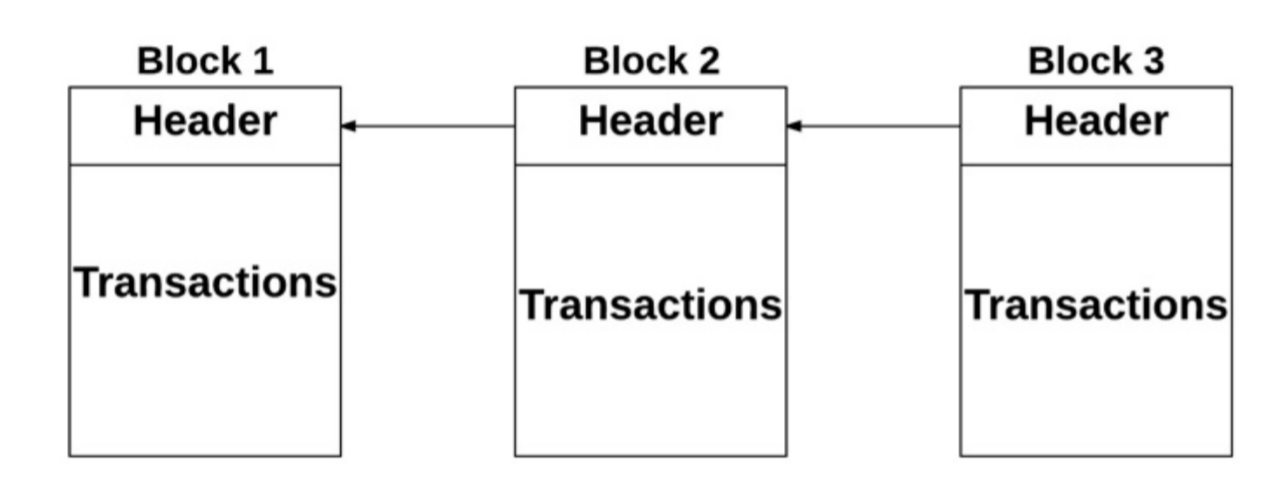
\includegraphics[scale=0.3]{blockchain.png}
	\caption{Structure of a Blockchain}
\end{figure}

\paragraph{}A node will periodically collect
multiple transactions from its pool of pending transactions toform a block, which is broadcast to the entire network. The
block is appended to the local copy of the BC stored at a node
if all constituent transactions are valid. A consensus algorithm
such as Proof of Work (PoW), which involves solving a hardto-
solve easy-to-verify puzzle, is employed to control which
nodes can participate in the BC. Once a block is appended, it
(or the constituent transactions) cannot be modified, since the
hash of each block is contained in the subsequent block in the
chain, which ensures immutability. A node can change its PK
(i.e. identity) after each transaction to ensure anonymity and
privacy.
\section{Blockchain}
\paragraph{}Current online transaction rely on certain trusted
institutions. However, these third party sources can be hacked,
manipulated or compromised[5] . Thus, novel secure schemes
are required.
In 2008, Nakamoto Satoshi proposed the Blockchain
technology to solve the above problems. They explain
electronic cash which is dealt in peer-to-peer network so that
direct transactions can be made between the two parties
without trading through a third trusted institution. A
Blockchain is essentially a public ledger that is executed and
shared between participants.

\begin{figure}[H]
	\centering
	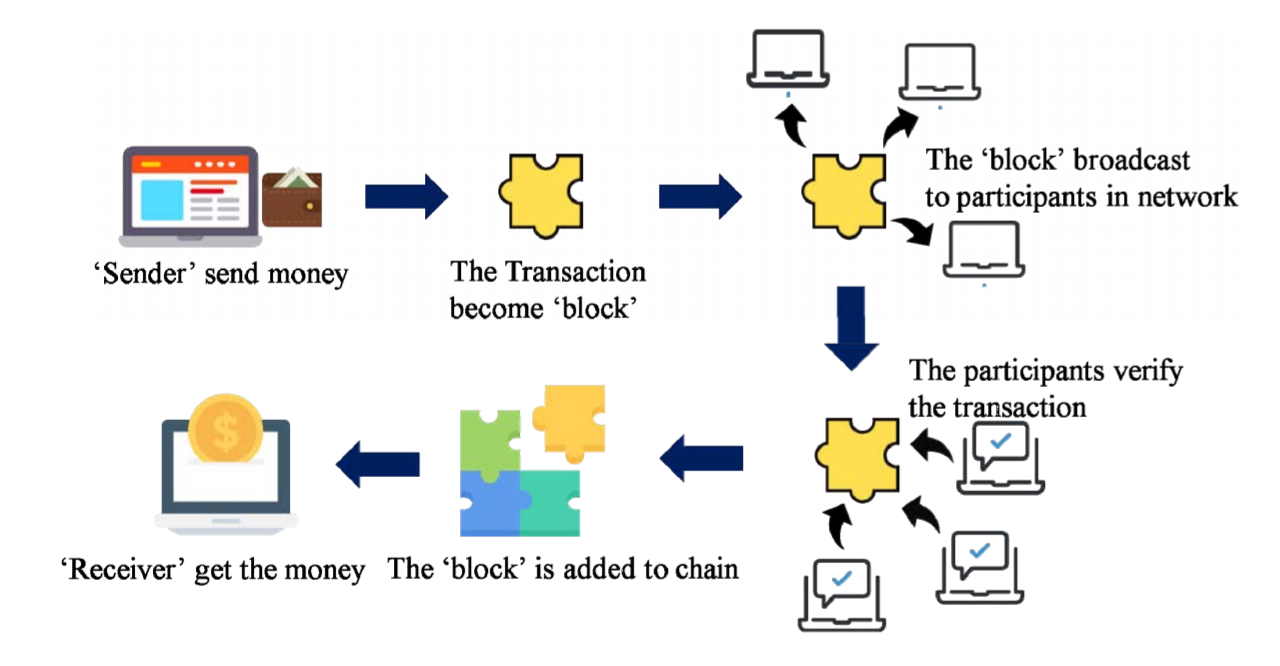
\includegraphics[scale=0.3]{working_blockchain.png}
	\caption{How Blockchain Works}
\end{figure}

\paragraph{}
 Once the data has been entered
into the block, it is difficult to forge or delete the information.
If a malicious user attempts to modify or delete a block, it must
also modify all previous blocks as well as the block at that
point in time. The Figure shows an example of an online
transaction using Blockchain. Each Blocks constituting a Blockchain consist of a 'block
header' and a 'block body'. The block header includes the hash
value of the previous block header. In addition, each block is
linked by a linked list method such as a chain. Block bodies
may contain different values depending on its service.
\section{Simplified Payment Verification - SPV}
\paragraph{}Note that all nodes do not possess the capability to store the
full Blockchain especially the resource constrained devices,
e.g., space and power-constrained devices cannot maintain the
full Blockchain. Therefore, for such devices, a simplified
payment verification (SPV) is used to operate without the full
Blockchain. SPV nodes download only the block header rather
than the complete chain. Therefore, they do not know about the
transactions.
SPV nodes can verify the transactions using a different
method. They verify transactions by reference to their depth in
the Blockchain instead of the height. SPV nodes will verify the
chain of all blocks and link that specific chain to the
transaction of interest . The SPV node will establish a link
between the transaction and the block that contains it, using a
Merkle Path.


\begin{figure}[H]
	\centering
	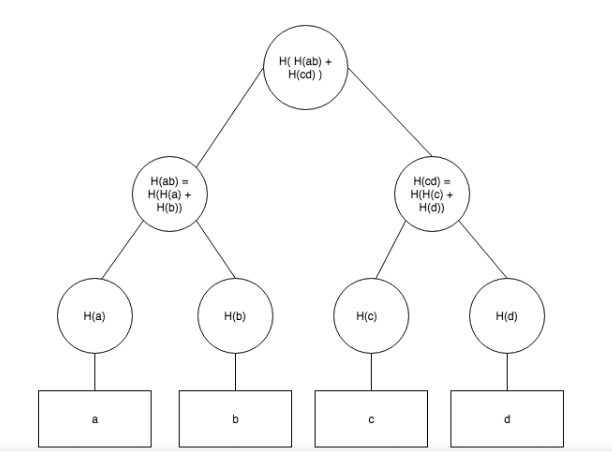
\includegraphics[scale=0.5]{merkle_path.png}
	\caption{Merkle Path}
\end{figure}


\paragraph{}a, b, c, and d are some data elements (files, public/private keys, JSON, etc) and H is a hash function. If you are unfamiliar, a hash function acts as a “digital fingerprint” of some piece of data by mapping it to a simple string with a low probability that any other piece of data will map to the same string. Each node is created by hashing the concatenation of its “parents” in the tree. You will notice that the Merkle tree here is a binary tree, most Merkle Trees are binary, but there are non-binary Merkle Trees employed in platforms like Ethereum. Here I will just cover the binary case as it is by far the most common.
\paragraph{}
The tree can be constructed by taking nodes at the same height, concatenating their values, and hashing the result until the root is reached. A special case needs handled when only one node remains before the tree is complete, but other than that the tree construction is somewhat straightforward (more on this in the implementation section).
\paragraph{}
Once built, data can be audited using only the root hash in logarithmic time to the number of leaves (this is also known as a Merkle-Proof). Auditing works by recreating the branch containing the piece of data from the root to the piece of data being audited. In the example above, if we wanted to audit c (assuming I have the root hash), I would need to be given H(d) and H(H(a) + H(b)). I would hash c to get H(c), then concatenate and hash H(c) with H(d), then concatenate and hash the result of that with H(H(a) + H(b)). If the result was the same string as the root hash, it would imply that c is truly a part of the data in the Merkle Tree.
\paragraph{}
In a case such as torrenting, another peer would provide the piece of data, c, H(d), and H(H(a) + H(b)). If you’re concerned about the security of this approach, recall that in a hash function it is computationally infeasible find some e such that H(e) = H(c). This means that so long as the root hash is correct, it would be difficult for adversaries to lie about the data they were providing.
\paragraph{}
Outputting the authentication path of some data is as simple as recreating the branch leading up until the root. Traversing the entire tree to produce the leaves and their respective authentication data becomes important when using the Merkle Tree in digital signature schemes, and this can actually be accomplished in under logarithmic time.

\chapter{Scenarios and System Architecture}
\paragraph{}
The system consists of a
power supplier, a service provider, and a mobile charger. It is
assumed that both the Service Provider and the mobile charger
parent node are Full Block. The remaining mobile chargers
utilize SPV. In this section, I propose a data structure of a
mobile charger for charging through a mobile charger, and
discuss how to make lightweight Blockchain.

\begin{figure}[H]
	\centering
	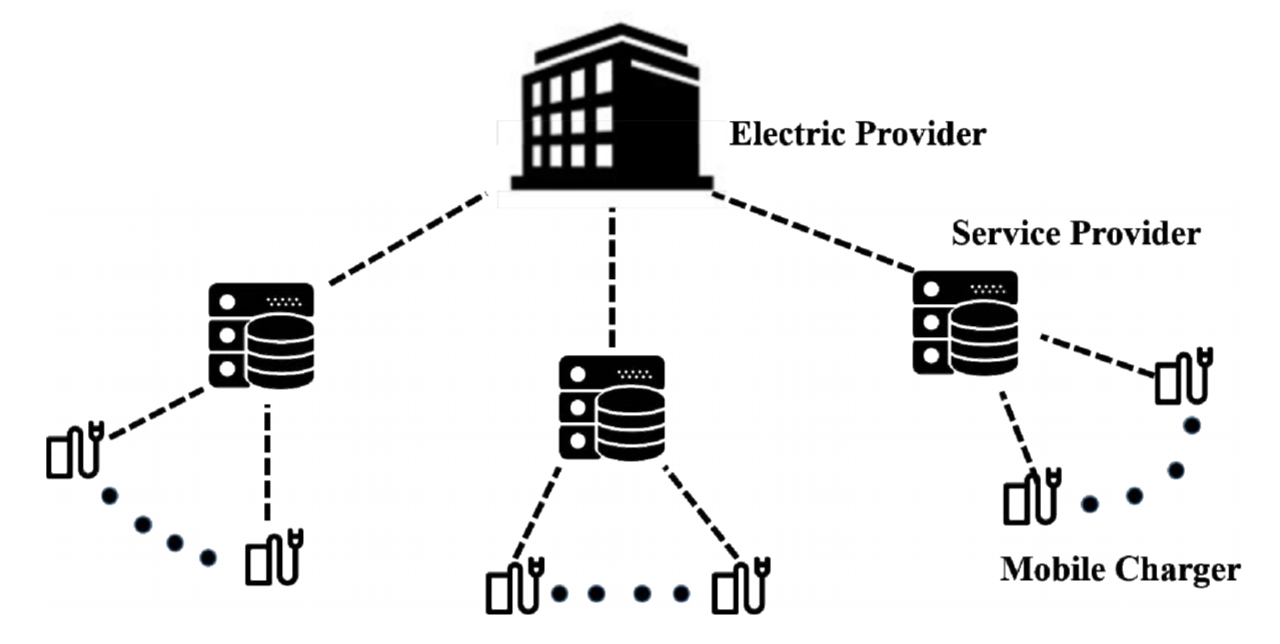
\includegraphics[scale=0.3]{system_model.png}
	\caption{System Model}
\end{figure}

\section{Mobile charger packet information for billing}

\paragraph{}
Before referring to the mobile charger packet information
for billing according to its charging, it is assumed that each
mobile charger knows the IP address of its own service
provider. If each mobile charger is operated on the network
for the first time, it can only participate if it searches other
nodes in the network. As this time, each mobile charger can
obtain the information of the current block and the
neighboring node through the service provider.

\paragraph{}
It shows the message type and data type of the mobile
charger. Table 4.1 shows the message type whereas the data
types are specified in Table 4.2. If some users make charging
group and pay the charging fee at the same time, it is much
more effective to impose one charger group than to charge for
each mobile chargers. Furthermore, some person group can
pay the charging fee at the same time, this case is same as like
the previous case. Therefore, the mobile charger can have a
‘groupId’ value with a unique identifier. If certain mobile
chargers are grouped together, they can be grouped by passing
their groupId value to their service provider.

\FloatBarrier
\begin{table}[h]
 \begin{center}
     \caption{ Message Type}
%\setlength{\arrayrulewidth}{1mm}
%\setlength{\tabcolsep}{18pt}
%\renewcommand{\arraystretch}{1.5}
\paragraph{}

\begin{tabular}{ |p{3cm}|p{9cm}| }
\hline
\bf Message  & \bf Description  \\
\hline
Register & The mobile charger registers itself by             
transferring its ‘idTag’ to the Service
Provider Server.If grouping is
required, the ‘groupId’ value can be
passed along with the idTag value  \\
\hline
RegisterAck & Response message to ‘Register’.   \\
\hline
CheckAuth & If a new mobile charger is added to the
group, the Service Provider server
forwards this message to the parent
node of the group. After receiving this
message, the mobile charger confirms
that the idTag value of the charger to
be added belongs to its own group.  \\
\hline
CheckAuthAck & Response message to ‘CheckAuth’   \\
\hline
Authorize  &  A mobile charger participating in a
group requests permission to join the
group by sending its idtag. \\
\hline
AuthorizeAck & Ack Response message to ‘Authorize’  \\
\hline
     \end{tabular}
   \end{center}
  \end{table}
\FloatBarrier

\paragraph{}
\paragraph{}


\FloatBarrier
\begin{table}[h]
 \begin{center}
     \caption{ Data Type}

%\setlength{\arrayrulewidth}{1mm}
%\setlength{\tabcolsep}{18pt}
%\renewcommand{\arraystretch}{1.5}
 
\paragraph{}

\begin{tabular}{ |p{3cm}|p{9cm}| }
\hline
\bf Type  & \bf Description  \\
\hline
idTag  & Mobile Charger unique identifier \\
\hline
idTagInfo  &  It is delivered after registration.
There are ‘Interval’, ‘currentTime’,
‘status’ fields. ‘status’ field is used only when
making a group, and if it has an
Accepted, it means the mobile
charger get authority to the group \\
\hline
Interval &  Cycle to send ‘ChargeProfile’ \\
\hline 
currentTime & The current time in the Service
Provider. It is used to synchronize the
mobile charger's internal clock \\
\hline
ChargeProfile & Charge history of mobile charger. It
consists of idtag and each charge
history. Charging history includes
start time, maximum output power,
and end time. \\
\hline
   \end{tabular}
   \end{center}
  \end{table}
\FloatBarrier

\paragraph{}Each message and description is shown in
Table 4.1. Each groupId value is unique, and the first mobile
charger to register groupId serves act as the ‘parent node’ of
the group. In the proposed system, the parent mobile charger is
a full node(all blocks are held), and the other mobile charger in
the group is an SPV node. The messages inlcudes Register, RegisterAck, CheckAuth, CheckAuthAck, Authorize. 

\paragraph{}Each data type and description is shown in
Table 4.2. Each idTag value is unique, which represents the unique identifier. The data type inlcudes idTag, idTagInfo, Interval, currentTime,ChargeProfile. 

\begin{figure}[H]
	\centering
	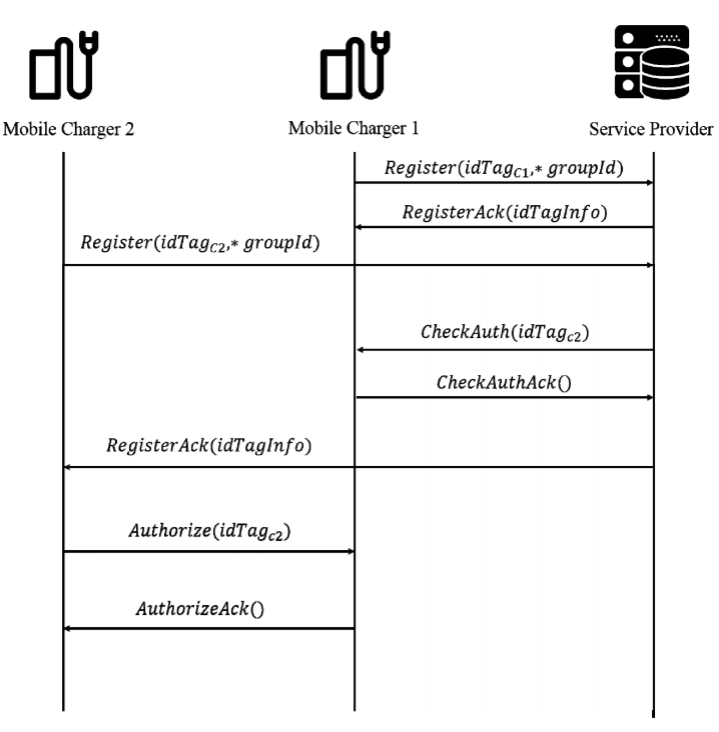
\includegraphics[scale=0.4]{charger_registration.png}
	\caption{Sequence of the mobile charger registration}
\end{figure}

\paragraph{}After completing the registration sequence with the Service
Provider, the mobile charger transmits its Charging Profile to
the Service Provider after completing the charging process. If
the service provider receives 'Charging Profile' from mobile
charger, it sends the 'Charging profile' to chargers belonging to
other group. The mobile charger delivers all its charging
profiles which occurred within the ‘interval’ value from
idTagInfo to the parent node.
\paragraph{}
The parent node that receives the
profile of the group generates a block containing the contents
of all profiles and sends it to the service provider. The Service
Provider forwards the block to all groups. If you get more than
half the correct validation results for a transaction, the service
provider adds the block to the existing Blockchain. Then
Service Provider pass the block to all nodes. The service
provider checks the block information for billing and transmits
the charge information according to the charge amount for each
group.

\begin{figure}[H]
	\centering
	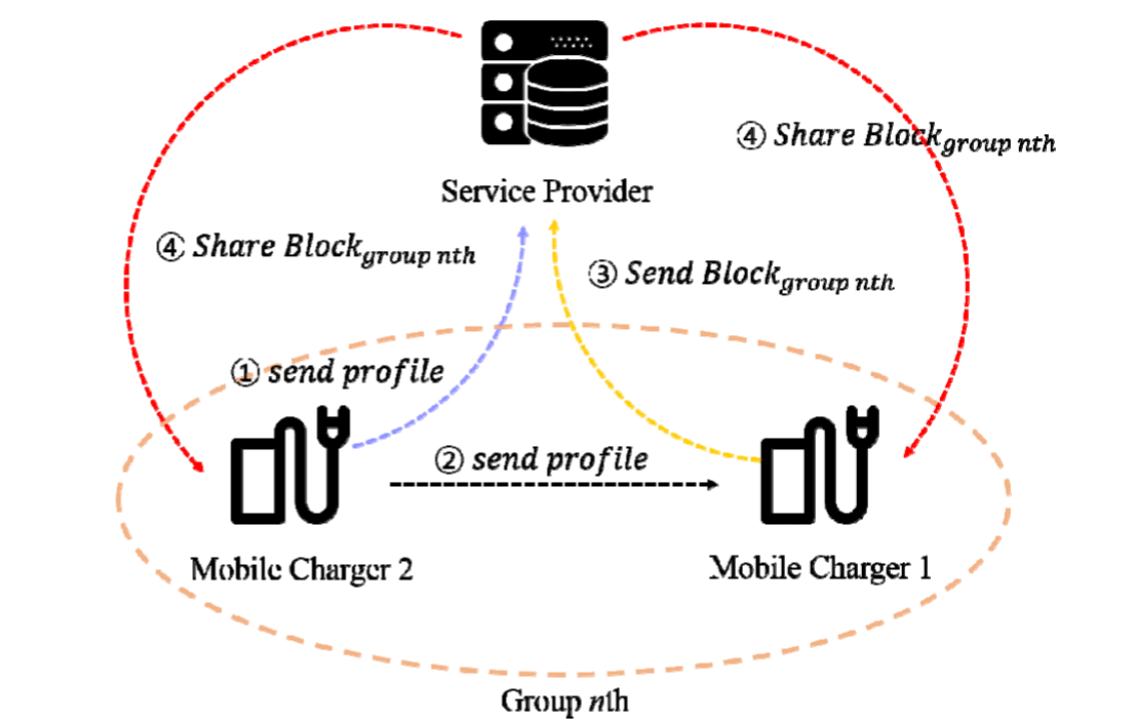
\includegraphics[scale=0.39]{transaction_communication.png}
	\caption{Sequence of Transaction Communication}
\end{figure}

\section{Lightweight Blockchain data}
\paragraph{}Currently, the Blockchain technique has some limitations.
One of the biggest challenge in it is the size of the data. The
Blockchain will continue to accumulate previous data records,
so the size of the data over time will increase. Moreover, in
Blockchain architecture the data is generated after every predetermined
period and this data is broadcasted to all node that
belong to the network. So, if the number of nodes are
increased, the data size will grow exponentially. Thus the cost
of maintaining this data will also increase accordingly.
\paragraph{}
To reduce the size of the data, a simple way is to delete the
old block data which are no longer needed and not required to
be maintained. However, this method may cause another issue
relating to the loss of the data value at a certain time. For
example, since the previous charge record is deleted, the user
may deny the its bill even though the charge was actually made
by the user.

\begin{figure}[H]
	\centering
	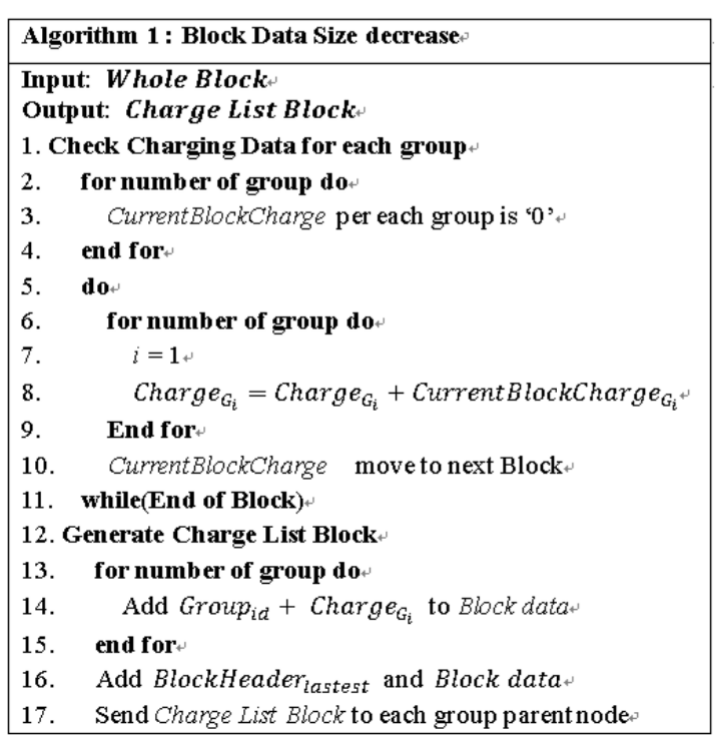
\includegraphics[scale=0.5]{algorithm.png}
	\caption{Algorithm - Block Data Size Decrease}
\end{figure}

\paragraph{}
In my proposed scheme, parent mobile charger maintains
the full Blockchain and other mobile chargers in the group are
SPV node. In such case, any charger may be reluctant to
become a parent node as the parent mobile charger have to
maintain an additional overhead of the full block. So, I
propose a novel method to reduce Blockchain data size for
parent node. The proposed method makes more efficient
management compared to the block data. The proposed method
is a re-construction of a block into a new type of block which is
called Charge List Block. The service provider receives block
for each group transaction from the parent node, and it reconstructs
the block body part.
\paragraph{}The service provider
periodically checks the size of the Blockchain data received
from each group. If the size of the Blockchain data exceeds a
certain size, it check the billing profile for the last transaction
for each group. The Service Provider checks the height of the
block from the first block to the block containing the last
transaction contents. After this process, the Service Provider
creates a Charge List Block by listing the idTag and charge
usage of all mobile chargers in the group. The block header of
the Charge List Block is generated in the same way as the
existing block header part, and is transmitted for each group.
The group parent mobile chargers receive the newly created
block form a new Blockchain starting from the reconstructed
block. Through this method, the parent mobile charger can be
maintained the lightweight full Blockchain.

\section{Performance Analysis}  

\paragraph{}In this section, I present the results of the analysis for the
proposed method of mobile chargers and the lightweight
Blockchain technique.If any malicious user wants to change the existing charging
record, he or she must change not only that block but also all
blocks after that block. In fact, it is impossible to change the
record because it is shared by all nodes participating in the
network.Since the parent node receives the profile in the group of
every interval, the malicious user may attempt to change the
value of the profile in the group on the parent node.
\paragraph{} This is
because, if the parent node changes the value to generate a
block, the nodes belonging to the other group receive the
existing profile contents in advance, and can confirm whether
or not the profile is changed through validation. If the contents
of the profile are different, the block containing the profile is
not tied to the existing Blockchain. Therefore, it is impossible
to attack a profile change with malicious parent.
The proposed lightweight Blockchain scheme can reduce
the size of existing Blockchain data.
\paragraph{} Existing blocks must
include a signature and a secret key for each transaction.
However, if the proposed method is used, the data size can be
greatly reduced because only the idTag, the charging amount
of the mobile charger and the hash of the last transaction are
maintained even if the number of transactions increases.


